\documentclass[12pt,aspectratio=169]{beamer}
\usetheme[dept=ai,coloredtitles,coloredblocks,copyright={}]{vub} % This will automatically load all fonts (Roboto and TeX Gyre Adventor
               % for titles), and the VUB colors. Also includes the triangle.
\title{A framework for step-wise explaining how to solve constraint satisfaction problems}
% \department{ai}
%\subtitle{Your subtitle} % Can be omitted
\usepackage{graphicx}
\usepackage{amsmath}
\usepackage{roboto}  %% Option 'sfdefault' only if the base font of the document is to be sans serif
\usepackage{fontenc}
\usepackage{amssymb}
\usepackage{amssymb}
\usepackage{xspace}
\newcommand\m[1]{\ensuremath{#1}\xspace}
\usepackage{natbib}

% \usepackage[dvipsnames]{xcolor}
\usepackage[ruled,linesnumbered]{algorithm2e}
% \newcommand\land\wedge
\newcommand\limplies\Rightarrow
\author{{\bf Bart Bogaerts} \\(Joint work with Emilio Gamba, Jens Claes, and Tias Guns)}
\date{April 20, 2021 @ Beyond Satisfiability}

% …


% \newtheorem{proposition}{Proop}

\begin{document}
\frame{\maketitle} % Automatic titlepage with VUB logo.



\section{Introduction: Beyond Satisfiability}
\begin{frame}{Beyond Satisfiability}
 \begin{itemize}
  \item ``There Are No CNF Problems'' (P.J. Stuckey) 
  \item Adopt a (simple) high-level modeling language  \pause
  \item Structural information of the problem visible
  \item E.g., symmetry breaking
  \begin{align*}& \forall p[Pigeon] \exists h [Hole]: In(p,h)\\
   &\forall h [Hole], p_1 p_2 [Pigeon]: In(p_1,h) \land In(p_2,h) \limplies p_1 = p_2.
  \end{align*}
  \pause
  \item Choice ... fragmentation ... ASP, CP, SMT, $\dots $
   \end{itemize}
\end{frame}

\begin{frame}{Beyond Satisfiability: This Talk}
\begin{itemize}
  \item Algorithms: SAT level
  \item Explanation: first-order level
 \end{itemize} 
\end{frame}

\AtBeginSection[]
  {
     \begin{frame}<beamer>
     \frametitle{Outline}
     \tableofcontents[currentsection]
     \end{frame}
  }

\section{History: The Holy Grail Challenge}

\begin{frame}{Logic Grid Puzzles}
 \begin{itemize}
  \item Set of clues
  \item Sets of entities that need to be linked
  \item Each entitity is linked to exactly one entity of each other type (bijectivity)
  \item The links are consistent (transitivity)
 \end{itemize}
\end{frame}


\begin{frame}{Logic Grid Puzzles: Example}
 \begin{itemize}
  \item The person who ordered capellini paid less than the person who chose arrabiata sauce
\item The person who ordered tagliolini paid more than Angie
\item The person who ordered tagliolini paid less than the person who chose marinara sauce
\item Claudia did not choose puttanesca sauce
\item The person who ordered rotini is either the person who paid \$8 more than Damon or the person who paid \$8 less than Damon
\item The person who ordered capellini is either Damon or Claudia
\item The person who chose arrabiata sauce is either Angie or Elisa
\item The person who chose arrabiata sauce ordered farfalle
 \end{itemize}
\end{frame}



\begin{frame}{2019 Holy Grail Challenge: Logic Grid Puzzles}
 \begin{itemize}
    \item Parse puzzles and translate into CSP
    \item Solve CSP automatically
    \item Explain in a human-understandable way how to solve this puzzle
 \end{itemize}
 \pause
 We won the challenge...
\pause
out of two participants 
 
\end{frame}


\begin{frame}{Demo}
 \begin{itemize}
   \item Automatically generated constraint representation from natural language (no optimization of the constraints for the explanation problem)
   \item No modifications to the underlying solvers (we do not equip each propagator with explanation mechanisms)
   \item demo:   \url{https://bartbog.github.io/zebra/pasta/}
 \end{itemize}

\end{frame}







\section{Step-Wise Explanations (ECAI 2020) } 
\begin{frame}{ECAI 2020 paper}
\begin{itemize}
\item Formalize the step-wise explanation problem
 \item Propose an algorithm (agnostic of actual propagators, consistency level, etc.) 
 \item Propose heuristics for guiding the search for explanations
 \item Experimentally demonstrate feasibility
\end{itemize}
 \end{frame}
 
 \begin{frame}{Preliminaries/Notation}
  \begin{itemize}
   \item Propositional vocabulary $\Sigma$
   \item (partial) interpretation $I$: consistent set of literals over $\Sigma$ \\
   \textit{Slightly abusing notation}: set of (unit) clauses
   \item Propositional theory $T$ (set of constraints over $\Sigma$) \\
      \textit{Slightly abusing notation}: set of constraints = conjunction
   \item Notation $T \land I \models I'$  
  \end{itemize}

 \end{frame}
 
 \newcommand\Iend{\m{I_{\mathit{end}}}}
 \begin{frame}{Goal}
   \begin{itemize}
    \item Given $T$ and $I$, let $\Iend$ denote the maximal set of literals such that 
    \[T \land I \models \Iend\]
    \item Explain in simple steps how to derive \Iend
    \item Our focus: single steps  (not optimizing entire sequence yet)
   \end{itemize}
 
 \end{frame}


 
 
 
 
\begin{frame}{Formalizing Explanations}
 \begin{definition}
 Let $I_{i-1}$ and $I_i$ be partial interpretations such that $I_{i-1}\wedge T \models I_i$.
 We say that $(E_i,S_i,N_i)$ \emph{explains} the derivation of $I_{i}$ from $I_{i-1}$ if the following hold:
\begin{itemize}
    \item $N_i= I_i \setminus I_{i-1}$ (i.e., $N_i$ consists of all newly defined facts), 
	\item $E_i\subseteq I_i$ (i.e., the explaining facts are a subset of what was previously derived),
	\item $S_i \subseteq T$ (i.e., a subset of the clues and implicit constraints are used), and 
	\item $S_i \land E_i \models N_i$ (i.e., all newly derived information indeed follows from this explanation).
\end{itemize}
\end{definition}
\end{frame}

\begin{frame}{Formalizing Explanations}
 \begin{definition}
 We call $(E_i,S_i,N_i)$ a \emph{non-redundant explanation of  the derivation of $I_i$ from $I_{i-1}$} if it explains this derivation and whenever $E'\subseteq E_i; S'\subseteq S_i$ while $(E',S',N_i)$ also explains this derivation, it must be that $E_i=E', S_i=S'$. 
\end{definition}
\pause
Observation: computing non-redundant explanations of a single literal can be done using Minimal Unsat Core (MUS) extraction:
\begin{theorem}
  There is a one-to-one correspondence between $\subseteq$-minimal unsatisfiable cores of $I_i\land T\land \lnot \ell$ and non-redundant explanations of $I_i\cup\{\ell\}$ from $I_i$ (given $T$).
\end{theorem}

\end{frame}






\begin{frame}{Formalizing Explanations}
 \begin{definition}
 We call $(E_i,S_i,N_i)$ a \emph{non-redundant explanation of  the derivation of $I_i$ from $I_{i-1}$} if it explains this derivation and whenever $E'\subseteq E_i; S'\subseteq S_i$ while $(E',S',N_i)$ also explains this derivation, it must be that $E_i=E', S_i=S'$. 
\end{definition}
% \pause
Furthermore, we assume existence of a \emph{cost function} $f(E_i,S_i,N_i)$ that quantifies the interpretability of a single explanation
\end{frame}


\begin{frame}{Formalizing Explanations}
\begin{definition}
Given a theory $T$ and initial partial interpretation $I_0$, the \emph{explanation-production problem} consist of finding a non-redundent explanation sequence
\[(I_0,(\emptyset,\emptyset,\emptyset)), (I_1,(E_1,S_1,N_i)), \dots ,(I_n,(E_n,S_n,N_n))\]
such that some aggregate over the sequence $\left(f(E_i,S_i,N_i)\right)_{i\leq n}$ is minimised.
\end{definition} 
\end{frame}

\newcommand\call[1]{\m{\textsc{#1}}}
\newcommand\onestep{\call{OneStep}}

\begin{frame}{MUS-Based Explanation Generation}
%  TODO ALGORITHM FROM IJCAI MUS... 
 
\begin{algorithm}[H]
  \caption{$\onestep(T,f,I,\Iend)$}
  \label{alg:oneStep}
$X_{best} \gets \mathit{nil}$\;
\For{$\ell \in \{\Iend \setminus I\}$}{
    $X \gets \call{MUS}{(T \land I \land \neg \ell)}$\;
    \If{$f(X)<f(X_{best})$}{
        $X_{best} \gets X$\;
    }
}
\Return{$X_{best}$} 
\end{algorithm}

\end{frame}


\begin{frame}{MUS-based Generation not sufficient} 
 \begin{itemize}
  \item MUS guarantees non-redundancy ... 
  \item ... does not guarantee quality
  \pause
  \item ECAI paper: MUS-based workaround (heuristic): do not use full $T$, but approximate
  \pause
  \item No details in this talk.
 \end{itemize}

\end{frame}


\begin{frame}{Implementation (ECAI paper)}
 \begin{itemize}
%   \item 
 \item Visual explanation interface
 \item Logic Grid puzzle cost function: 
 \begin{itemize}
 \item Single implicit axiom: very cheap
 \item Single constraint + implicit: less cheap
 \item Multiple constraints: very expensive
 \end{itemize}
 \pause {  \centering 

 ``The person who ordered capellini is either Damon or Claudia''. 
\[\exists p: ordered(p,capellini)\land (p = Damon\lor p = Claudia).\]}
\pause 
%  \item (demo) 
  \item Under the hood: IDP system \cite{IDP} %(ASP-like) 
\end{itemize}


\end{frame}





\section{The OCUS Problem (Hitting Set--Based Algorithms) (Under Review)} 


\begin{frame}{Beyond MUS-based explanations}
 \begin{itemize}
  \item MUS: $\subseteq$-minimal
  \item SMUS: $\#$-minimal (still not sufficient...) 
  \pause
  \item New problem OUS
 \end{itemize}
\end{frame}


\newcommand\nat{\m{\mathbb{N}}}
 \newcommand\formula{\m{T}}
 \newcommand\subsetT{\m{\mathcal{S}}}
 \newcommand\ltrue{\m{\textbf{t}}}
 \newcommand\lfalse{\m{\textbf{f}}}
% 

\begin{frame}{The OUS problem}
\begin{definition}
   Let $T$ be a formula, $f:2^{T} \to \nat$ a cost function. We call %a set $U\subseteq \formulag$ a \emph{$p$-constrained $f$-OUS} of \formulag ($(p,f)$-OUS) \tias{what with the OCUS name here?} \bart{I propsoe to say. We call 
    $\mathcal{S} \subseteq T$ an OUS of $T$ (with respect to $f$) if \begin{itemize}                                      
      \item $\subsetT$ is unsatisfiable,
%       \item $p(\subsetT)$ is true
      \item all other unsatisfiable $\mathcal{S}'\subseteq T$ satisfy $f(\mathcal{S}')\geq f(\mathcal{S})$.
    \end{itemize}
\end{definition}
\pause
\textbf{Q}: How to compute OUSs?
\end{frame}

\begin{frame}{OUS-Based Explanation Generation}
%  TODO ALGORITHM FROM IJCAI MUS... 
 
\begin{algorithm}[H]
  \caption{$\onestep(T,f,I,\Iend)$}
  \label{alg:oneStep}
$X_{best} \gets \mathit{nil}$\;
\For{$\ell \in \{\Iend \setminus I\}$}{
    $X \gets \call{OUS}{(T \land I \land \neg \ell)}$\;
    \If{$f(X)<f(X_{best})$}{
        $X_{best} \gets X$\;
    }
}
\Return{$X_{best}$} 
\end{algorithm}

\end{frame}

\begin{frame}{Beyond OUS-based explanations}
 \begin{itemize}
  \item The different iterations (for loop line 2)... very similar
  \item Can we exploit this? 
  \pause
  \item Essentially, the task at hand is: find a single unsatisfiable subset of 
  \[T\land I \land \bigvee_{\ell\in \Iend\setminus I}\lnot \ell\]
  that:
  \begin{itemize}
   \item Is optimal w.r.t.\ $f$
   \item Contains \emph{exactly one} literal $\lnot \ell$ with $\ell \in \Iend\setminus I$ (\emph{example!})
  \end{itemize}

 \end{itemize}

\end{frame}

% 

% 
%    Let $\formula$ be a formula, $f:2^{\formula} \to \nat$ a cost function and  $p$ a predicate $p: 2^{\formula}\to \{\ltrue,\lfalse\}$. We call %a set $U\subseteq \formulag$ a \emph{$p$-constrained $f$-OUS} of \formulag ($(p,f)$-OUS) \tias{what with the OCUS name here?} \bart{I propsoe to say. We call 
%  $\subsetT \subseteq \formula$ an OCUS of \formula (with respect to $f$ and $p$) if \begin{itemize}                                      
%       \item $\subsetT$ is unsatisfiable,
%       \item $p(\subsetT)$ is true
%       \item all other unsatisfiable $\subsetT'\subseteq \formula$ with $p(\subsetT')=\ltrue$ satisfy $f(\subsetT')\geq f(\subsetT)$.
%     \end{itemize}
% 
 \begin{frame}{The OCUS problem}
 \begin{definition}
   Let $\formula$ be a formula, $f:2^{\formula} \to \nat$ a cost function and  $p$ a predicate $p: 2^{\formula}\to \{\ltrue,\lfalse\}$. We call %a set $U\subseteq \formulag$ a \emph{$p$-constrained $f$-OUS} of \formulag ($(p,f)$-OUS) \tias{what with the OCUS name here?} \bart{I propsoe to say. We call 
    $\subsetT \subseteq \formula$ an OCUS of \formula (with respect to $f$ and $p$) if \begin{itemize}                                      
      \item $\subsetT$ is unsatisfiable,
      \item $p(\subsetT)$ is true
      \item all other unsatisfiable $\subsetT'\subseteq \formula$ with $p(\subsetT')=\ltrue$ satisfy $f(\subsetT')\geq f(\subsetT)$.
    \end{itemize}
\end{definition}
\end{frame}


\newcommand\onestepo{\ensuremath{\call{explain-One-Step-ocus}}\xspace}
\begin{frame}{OCUS-Based explanation generation}
 \begin{algorithm}[H]
  \DontPrintSemicolon
  \caption{$\onestepo(T,f,I,\Iend)$}
  \label{alg:oneStepOCUS}
  $p \leftarrow$ exactly one of $\overline{\Iend\setminus I}$\;
  \Return{$\call{OCUS}(T\land I\land \overline{\Iend\setminus I}, f, p)$} 
\end{algorithm}
\end{frame}


\newcommand\muses[1]{\m{\textsc{mus}s(#1)}}
\newcommand\mcses[1]{\m{\textsc{mcs}s(#1)}}
\begin{frame}{How to find OCUSs?}
 \begin{itemize}
  \item Hitting set--based algorithms: used for MaxSAT and SMUS 
%   \item We extended this idea to OCUS

\begin{theorem}\label{prop:MCS-MUS-hittingset}
%     Given an $ \formula$, let MUSes($\formula$), be the Minimal Unsatisfiable Subsets of F and MCSes($\formula$), be the Minimal Correction Subsets of F:
%     
    A set  $\subsetT \subseteq \formula$ is a MCS of $ \formula$ iff  it is a \emph{minimal hitting set} of \muses{\formula}.
% 
%     \noindent
    A set  $\subsetT \subseteq \formula$ is a MUS of $ \formula$ iff  it is a \emph{minimal hitting set} of \mcses{\formula}.
\end{theorem}
\pause
\item We extended this to OCUS: 
\end{itemize}

\end{frame}

\newcommand\setstohit{\m{\mathcal{H}}}
\newcommand\grow{\call{grow}}
\newcommand\sat{\call{SAT}}
\newcommand\comus{\call{ocus}}
\newcommand\cohs{\call{cost-optimal-hittingset}}

\begin{frame}{Hitting set--based OCUS}
 \begin{algorithm}[H]
  \DontPrintSemicolon
  $\setstohit  \gets \emptyset$ \; %\label{omus-line1} 
  \While{true}{
    $\subsetT \gets \cohs(\setstohit,f,p) $  \;%\tcp*{\small Find \textb    $\setstohit  \gets \setstohit  \cup \{  \formula \setminus \F''\}$ \;
% f{optimal} solution}
    % \tcp{\small set with all unique clauses from hitting set}
%     (sat?, $\kappa$) $\gets$ \texttt{SatSolver}($hs$)\;
    % \tcp{If SAT, $\kappa$ contains the satisfying truth assignment}
    % \tcp{IF UNSAT, $hs$ is the OUS }
    \If{ $\lnot \sat(\subsetT)$}{
      \Return{$\subsetT$} \;
    }
    $\subsetT \gets  \grow(\subsetT,\formula) $ \label{line:grow}\;
    $\setstohit  \gets \setstohit  \cup \{  \formula \setminus \subsetT\}$ \;
  }
  \caption{$\comus(\formula,f,p)$ }
  \label{alg:comus}
\end{algorithm}
\end{frame}

\newcommand\hitset{\m{\mathcal{H}}}

\begin{frame}{Correctness}
 \begin{theorem}\label{thm:soundcomplete}
  Let $\hitset$ be a set of correction subsets of \formula. 
  If $\subsetT$ is a hitting set of \hitset that is $f$-optimal among the hitting sets of \hitset satisfying a predicate $p$, and  $\subsetT$ is unsatisfiable, then $\subsetT$ is an OCUS of \formula. 
  
  If  $\hitset$ has no hitting sets satisfying $p$, then $\formula$ has no OCUSs.
\end{theorem}
\end{frame}

\begin{frame}{Two further ideas}
\begin{itemize}
 \item \emph{Incrementality}: re-use previous computations in future calls 
 \item \emph{Grow}: Develop implementations of ``grow'' tailored for explanations
\end{itemize}
 
\end{frame}

\begin{frame}{Incrementality}
 \begin{algorithm}[H]
  \DontPrintSemicolon
 {\bf  $\setstohit  \gets \dots$} \; %\label{omus-line1} 
  \While{true}{
    $\subsetT \gets \cohs(\setstohit,f,p) $  \;%\tcp*{\small Find \textb    $\setstohit  \gets \setstohit  \cup \{  \formula \setminus \F''\}$ \;
% f{optimal} solution}
    % \tcp{\small set with all unique clauses from hitting set}
%     (sat?, $\kappa$) $\gets$ \texttt{SatSolver}($hs$)\;
    % \tcp{If SAT, $\kappa$ contains the satisfying truth assignment}
    % \tcp{IF UNSAT, $hs$ is the OUS }
    \If{ $\lnot \sat(\subsetT)$}{
      \Return{$\subsetT$} \;
    }
    $\subsetT \gets  \grow(\subsetT,\formula) $ \label{line:grow}\;
    $\setstohit  \gets \setstohit  \cup \{  \formula \setminus \subsetT\}$ \;
  }
  \caption{$\comus(\formula,f,p)$ }
  \label{alg:comus}
\end{algorithm}
\end{frame}

\begin{frame}{Different Grow strategies}
 When calling OCUS, the theory consists of 
 \begin{enumerate}
  \item The original theory (constraints)\hfill \emph{$T$}
  \item The current interpretation\hfill \emph{$\Iend$}
  \item The negation of literals in $\Iend$  \hfill \emph{$\overline{\Iend}$}
 \end{enumerate}
 
 \begin{itemize}
  \item What to take into account for \emph{\call{grow}}?
  \item What about the cost function?
 \end{itemize}


 

\end{frame}

\begin{frame}{Experiments}
Implementation building on pysat + cpMpy 
\begin{description}
 \item[Q1] What is the effect of requiring optimality of the generated MUSs on the \textbf{quality} of the generated explanations?
 \item[Q2] Which \textbf{domain-specific \grow methods} perform best?
 \item[Q3] What is the effect of the use of \textbf{contrainedness} on the time required to compute an explanation sequence?
 \item[Q4] Does \textbf{re-use} of computed satisfiable subsets improve efficiency?
\end{description}
\end{frame}


\begin{frame}{Experiments: Solution Quality}
%  \begin{figure}[H]
  \centering
  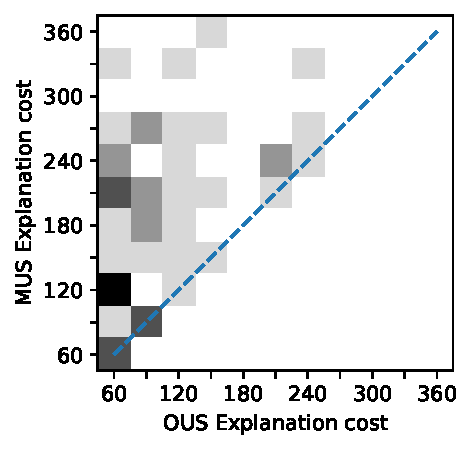
\includegraphics[width=0.54\columnwidth]{figures/rq1_heatmap.pdf}
%   \caption{Q4 - Grow strategies until timeout or full explanation sequence generation}
%   \label{fig:rq1_heatmap}
% \end{figure}
\end{frame}

\begin{frame}{Experiments: Grow Strategies}
  \centering
   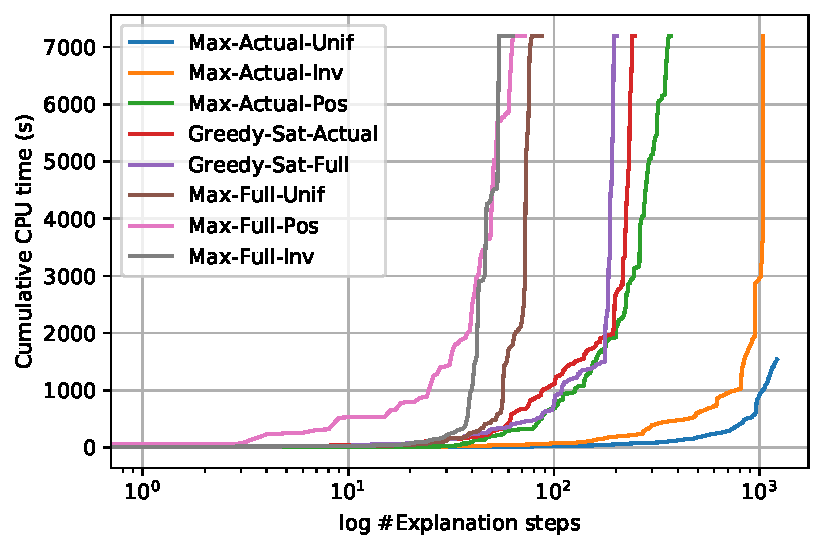
\includegraphics[width=0.8\columnwidth]{figures/loggrowWithSubsetmax.pdf}

\end{frame}

\begin{frame}{Experiments: Performance }
  \centering
  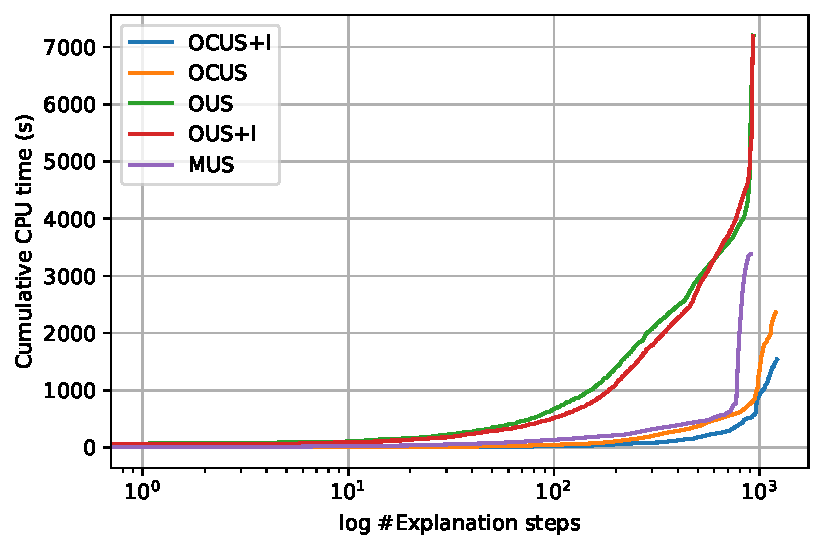
\includegraphics[width=0.8\columnwidth]{figures/rq4_b.pdf}

\end{frame}











\section{Nested Explanations (AIJ 2021)}

\begin{frame}{Observation}
 \begin{itemize}
  \item Some steps still quite difficult. 
   \item Idea: explanations at different levels of abstraction
  \item Explain hardest steps of the sequence
%   \pause
 \end{itemize}

\end{frame}

\begin{frame}{Example}
  \centering
  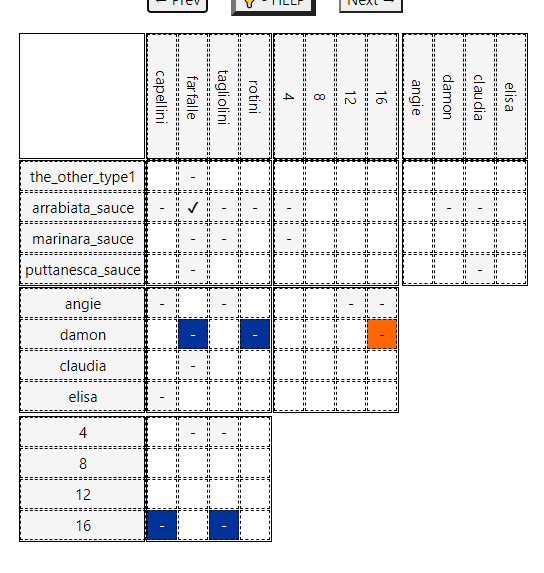
\includegraphics[width=0.4\columnwidth]{figures/difficult.png}
\end{frame}




\begin{frame}{Nested Explanations}
\begin{itemize}
   \item Idea: explanations at different levels of abstraction
  \item Counterfactual reasoning/proof by contradiction
  \item See demo \url{https://bartbog.github.io/zebra/pasta/}
%   \item Explain (counterfactual/towards contrad
\pause
\item For which steps? Hardest step of the nested sequence simpler than the step to explain
\end{itemize}
  
\end{frame}


\section{Conclusion}








\begin{frame}{Conclusion}
  \begin{itemize}
    \item Overview of a (relatively young) research project\\
    \qquad\ \qquad$\Rightarrow$ \emph{Lots of open questions!}
    \item \emph{Goal:}  Provide human-understandable explanations of inferences made by a constraint solver 
    \item Our \emph{proposal}: split in small comprehensible steps
    \item Explain them at different \emph{levels of detail} (abstraction)
    \item Triggers \emph{novel algorithmic needs}
    \item \emph{Demonstrated} on logic grid puzzles
  \end{itemize}

\end{frame}


% \begin{frame}{About this talk}
%  \begin{itemize}
%    \item 
%    \item Lots of open questions
%  \end{itemize}
% 
% \end{frame}

% \begin{frame}{Motivation}
% \begin{itemize}
%  \item Our take on \emph{explainable AI}
%  \item Context: Constraint solving
%  \item  %Explain (strong, complex) propagation in simple steps
%  \item Interactive constraint solving
% \end{itemize}
% 
% \end{frame}
% 
% \begin{frame}{History}
% \begin{itemize}
%  \item 2019 Holy Grail Challenge: Logic Grid Puzzles
%  \begin{itemize}
%     \item Parse puzzles and translate into CSP
%     \item Solve CSP automatically
%     \item Explain in a human-understandable way how to solve this puzzle
%  \end{itemize}
%  \item More generic paper at ECAI 2020 \cite{ecai2020}
%  \item Journal version and follow-up conference paper under review.
% \end{itemize}
% 
% \end{frame}
% 
% \begin{frame}{What we worked on already }
% \begin{itemize}
%  \item Formalize the step-wise explanation problem
%  \item Propose an algorithm (agnostic of actual propagators, consistency level, etc.) 
%  \item Propose heuristics for guiding the search for explanations
%  \item Experimentally demonstrate feasibility
%  \item (unpublished) Nested explanations (conceptual extension)
%  \item (unpublished) Incremental OMUS algorithms (efficiency bottleneck) 
% \end{itemize}
% \end{frame}
% 
% 
% % 
% % 
% % \begin{frame}{Logic Grid Puzzles}
% %  \begin{itemize}
% %   \item Set of clues
% %   \item Sets of entities that need to be linked
% %   \item Each entitity is linked to exactly one entity of each other type (bijectivity)
% %   \item The links are consistent (transitivity)
% %  \end{itemize}
% % \end{frame}
% 
% 
% % \begin{frame}{Logic Grid Puzzles}\centering
% % \hspace*{-30pt}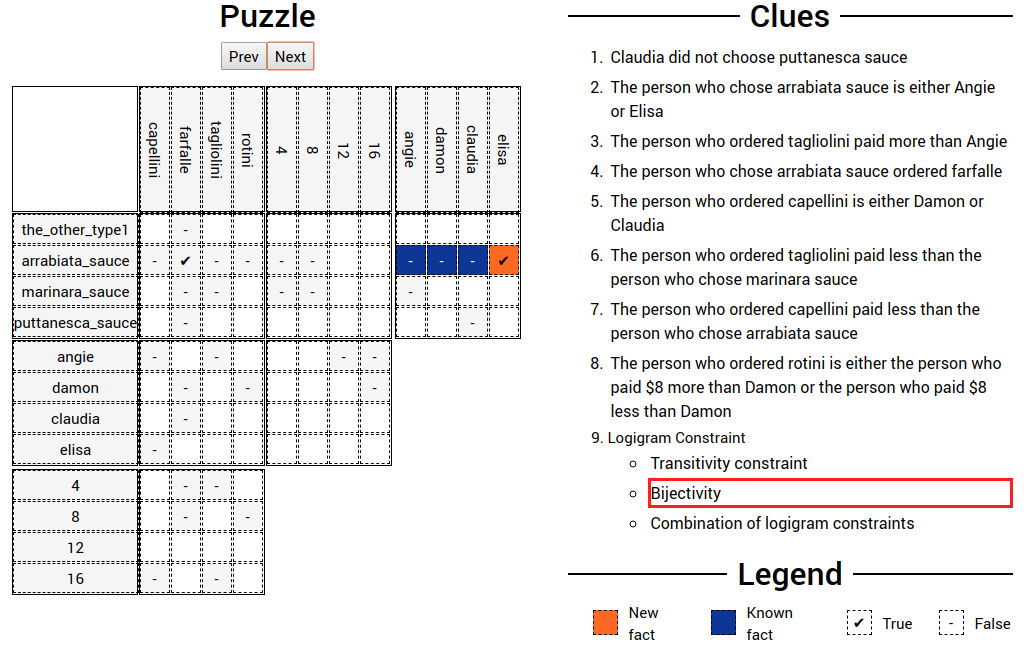
\includegraphics[width=1.2\textwidth]{zebra_screen.png} 
% %  \end{frame}
% % \end{frame}
% % \begin{frame}{Some terminology}
% % \[\begin{tabular}{ll}
% %   Logic & Constraint Programming \\
% %     \hline
% %   (partial) interpretation & (partial) assignment\\
% %   theory & model\\
% %   model & solution/satisfying assignment
% % \end{tabular}
% % \]
% % 
% % I will use propositional logic for the formalization: Boolean variables; interpretations are sets of literals, ... 
% %   
% % \end{frame}
% 
% 
% \begin{frame}{Problem}
%  \begin{definition}
%  Let $I_{i-1}$ and $I_i$ be partial interpretations such that $I_{i-1}\wedge T \models I_i$.
%  We say that $(E_i,S_i,N_i)$ \emph{explains} the derivation of $I_{i}$ from $I_{i-1}$ if the following hold:
% \begin{itemize}
%     \item $N_i= I_i \setminus I_{i-1}$ (i.e., $N_i$ consists of all newly defined facts), 
% 	\item $E_i\subseteq I_i$ (i.e., the explaining facts are a subset of what was previously derived),
% 	\item $S_i \subseteq T$ (i.e., a subset of the clues and implicit constraints are used), and 
% 	\item $S_i \cup E_i \models N_i$ (i.e., all newly derived information indeed follows from this explanation).
% \end{itemize}
% \end{definition}
% \end{frame}
% 
% \begin{frame}{Problem}
%  \begin{definition}
%  We call $(E_i,S_i,N_i)$ a \emph{non-redundant explanation of  the derivation of $I_i$ from $I_{i-1}$} if it explains this derivation and whenever $E'\subseteq E_i; S'\subseteq S_i$ while $(E',S',N_i)$ also explains this derivation, it must be that $E_i=E', S_i=S'$. 
% \end{definition}
% \pause
% Observation: computing non-redundant explanations of a single literal can be done using Minimal Unsat Core (MUS) extraction:
% \begin{theorem}
%   There is a one-to-one correspondence between $\subseteq$-minimal unsatisfiable cores of $I_i\land T\land \lnot l$ and non-redundant explanations of $I_i\cup\{l\}$ from $I_i$.
% \end{theorem}
% 
% \end{frame}
% 
% \begin{frame}{Problem}
%  \begin{definition}
%  We call $(E_i,S_i,N_i)$ a \emph{non-redundant explanation of  the derivation of $I_i$ from $I_{i-1}$} if it explains this derivation and whenever $E'\subseteq E_i; S'\subseteq S_i$ while $(E',S',N_i)$ also explains this derivation, it must be that $E_i=E', S_i=S'$. 
% \end{definition}
% % \pause
% Furthermore, we assume existence of a \emph{cost function} $f(E_i,S_i,N_i)$ that quantifies the interpretability of a single explanation
% \end{frame}
% 
% 
% \begin{frame}{Problem}
% \begin{definition}
% Given a theory $T$ and initial partial interpretation $I_0$, the \emph{explanation-production problem} consist of finding a non-redundent explanation sequence
% \[(I_0,(\emptyset,\emptyset,\emptyset)), (I_1,(E_1,S_1,N_i)), \dots ,(I_n,(E_n,S_n,N_n))\]
% such that a predefined aggregate over the sequence $\left(f(E_i,S_i,N_i)\right)_{i\leq n}$ is minimised.
% \end{definition} 
% \end{frame}




\begin{frame}{Use cases}
 \begin{itemize}
  \item Teach humans how to solve a certain problem
  \item Quantify problem difficulty
  \item ``Help'' button
  \item Interactive configuration/planning/scheduling
 \end{itemize}

\end{frame}


% \begin{frame}{Next Steps: OMUS computation}
%   \begin{itemize}
%     \item Algorithms to compute Optimal MUSs 
%     \item Based on hitting-set duality
%     \item Combining existing SMUS (\#-minimal) \cite{SMUShit,DBLP:journals/constraints/IgnatievJM16} algorithms and MAXSAT \cite{davies} algorithms
%     \item \emph{Incremental} OMUS computation
%     \item \emph{Constrained} OMUS computation
%     \item No experimental results yet
%   \end{itemize}
% 
% \end{frame}

% 
% \begin{frame}
%   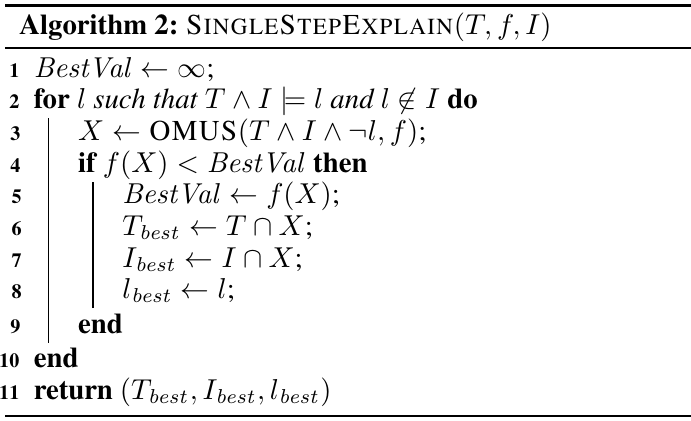
\includegraphics[width=\textwidth]{algo.png}
% \end{frame}
% 

\begin{frame}{Future work}
\begin{itemize}
%  \item Unsat-core optimization
 \item Learning the optimization function (from humans) -- Learning the level of abstraction
%  \item Nested explanation sequences
\item Explaining optimization (different types of ``why'' queries); close relation to Explainable AI Planning \cite{fox2017explainable}
\item Scaling up (approximate algorithms; decomposition of explanation search)
\item Incremental algorithms over different ``why'' queries
% \item 
\end{itemize}

 
\end{frame}

\begin{frame}{References}
% \tiny
\bibliographystyle{plain}
% \renewcommand*{\bibfont}{\footnotesize}
\def\bibfont{\footnotesize} 
% {\footnotesize 
\bibliography{refs.bib}
% }
\end{frame}


\end{document}
